\section{Решение} 


\subsection{Установка и настройка LSF}

Настройка значений полей в конфиг-файле \lstinline{install.config} \cite{install_plan}:
\begin{lstlisting}
LSF_ADMINS="lsfadmin"
LSF_TOP="/usr/share/lsf"
LSF_ADD_SERVERS="hostm hostb hostc hostd"
LSF_MASTER_LIST="hostm hostd"
LSF_ADD_CLIENTS="hoste hostf"
LSF_CLUSTER_NAME="cluster1"
CONFIGURATION_TEMPLATE="HIGH_THROUGHPUT"    
\end{lstlisting}

Пояснение полей:

\lstinline{LSF_ADMINS}: имена пользователей администраторов LSF;

\lstinline{LSF_TOP}: полный путь директории установки LSF;

\lstinline{LSF_ADD_SERVERS}: узлы, которые могут ставить задания в очередь и выполнять задания;

\lstinline{LSF_MASTER_LIST}: узел сервера LSF, который действует как всеобщий координатор для кластера. В каждом кластере есть один главный узел, который выполняет планирование и отправку всех заданий из очереди в узлы для выполнения;

\lstinline{LSF_ADD_CLIENTS}: узлы, которые могут только ставить задания в очередь;

\lstinline{LSF_CLUSTER_NAME}: имя кластера LSF;

\lstinline{CONFIGURATION_TEMPLATE}: шаблон конфигурации для определения начальной конфигурации нового кластера \cite{lsf_overview,host_types_models}.


Создание пользователя для администратора LSF и запуск установки LSF: 
\begin{lstlisting}
$ sudo -i
# adduser lsfadmin
# ./lsfinstall -f install.config
\end{lstlisting}

Запуск LSF:
\begin{lstlisting}
# source /usr/share/lsf/conf/profile.lsf
# lsfstartup
\end{lstlisting}


\subsection{Поддержка API для LSF в серверной части Scheduler}

За основу взяты шаблоны задач и скрипты bash системы очередей Torque для поддержки LSF. Шаблоны задач и скрипты Torque переписаны для LSF. Созданы скрипты bash

\lstinline{run_rnkim_decomp_mpi_lsf.sh},

\lstinline{run_rnkim_mpi_lsf.sh},

\lstinline{run_rnkim_omp_lsf.sh}

и шаблоны задач

\lstinline{template_rnkim_decomp_lsf},

\lstinline{template_rnkim_decomp_mpi_lsf},

\lstinline{template_rnkim_mpi_lsf},

\lstinline{template_rnkim_omp_lsf}

для LSF.

Переписывание скриптов bash с Torque на LSF:
{
\lstset{emph={job_file}, emphstyle=\itshape}
\begin{lstlisting}
qsub job_file
-->
bsub < job_file
\end{lstlisting}
}

Переписывание шаблонов задач с Torque на LSF:
\begin{lstlisting}
#PBS -l nodes=1_tmplNODETYPE_:ppn=_tmplCORES_
-->
#BSUB -n _tmplCORES_ -R "span[hosts=1]"
_tmplNODETYPE_


#PBS -l nodes=_tmplNNODES__tmplNODETYPE_:ppn=_tmplCORES_
-->
#BSUB -n _tmplTOTALCORES_ -R "span[ptile=_tmplCORES_]"
_tmplNODETYPE_

_tmplNODETYPE_="#BSUB -m \"$NODETYPE\""
TOTALCORES = NNODES * CORES


#PBS -m ea
#PBS -M <usermail>
-->
#BSUB -notify "exit done"
#BSUB -u <usermail>


#PBS -N _tmplMODEL_
#PBS -l walltime=150:00:00
#PBS -d _tmplDIR_
-->
#BSUB -J _tmplMODEL_
#BSUB -W 150:00
#BSUB -cwd _tmplDIR_
\end{lstlisting}


\subsection{Поддержка команд, направляемы напрямую из Scheduler на кластер}

Команды в Scheduler, относящиеся к конкретной системе очередей, хранятся в значениях ключей в словаре (тип данных на Python). Значениям соответствуют либо ссылки на исполняемые на сервере скрипты, либо команды для системы очередей, либо ссылки на методы обработки. Для LSF добавлены следующие значения:
\begin{lstlisting}
%Ключ%:                    %Значение%
QsysCMD.RUN_OMP:         "$RNKIMPATH/scripts/run_rnkim_omp_lsf.sh",
QsysCMD.RUN_MPI:         "$RNKIMPATH/scripts/run_rnkim_decomp_mpi_lsf.sh",
QsysCMD.RUN_MPI_ADV:     "$RNKIMPATH/scripts/run_rnkim_mpi_lsf.sh",
QsysCMD.DEL_TASK:        "bkill",
QsysCMD.GET_STAT:        "bjobs -json -o 'jobid user stat job_name submit_time start_time finish_time error_file output_file effective_resreq slots'",
QsysCMD.GET_STAT_MTHD:   lambda str_jobs: f"bjobs -json -o 'jobid user stat job_name submit_time start_time finish_time error_file output_file effective_resreq slots' {str_jobs}",
QsysCMD.PARSE_ID_MTHD:   lambda strout: int(strout[strout.find('<') + 1:strout.find('>')]),
QsysCMD.UPDT_JSTAT_MTHD: self._update_jstats_lsf
\end{lstlisting}

Метод \lstinline{_update_jstats_lsf} обновляет статус моделей. Парсит JSON статуса модели и вызывает метод \lstinline{_pars_job_json_lsf} для парсинга значений полей JSON статуса.

Метод \lstinline{_update_jstats_lsf} парсит поля с значениями у JSON статуса и записывает ключ 'имя модели' со значением словарь состояния:
\begin{lstlisting}
{
    "JOBID":"1363",
    "USER":"vagrant",
    "STAT":"EXIT",
    "JOB_NAME":"MODEL.DATA",
    "SUBMIT_TIME":"Jun  7 08:19",
    "START_TIME":"Jun  7 08:19",
    "FINISH_TIME":"Jun  7 08:19 L",
    "ERROR_FILE":"",
    "OUTPUT_FILE":"",
    "EFFECTIVE_RESREQ":"select[type == local] order[r15s:pg] span[ptile=2] ",
    "SLOTS":"2"
}
-->
model_name:
    {
        JobStat.ACC_NAME: str,
        JobStat.JOB_NAME: str,
        JobStat.OUT_PATH: str,
        JobStat.ERR_PATH: str,
        JobStat.JOB_STAT: ModelState,
        JobStat.NUM_NODES: int,
        JobStat.QUEUE_TIME: datetime,
        JobStat.START_TIME: datetime,
        JobStat.COMPL_TIME: datetime
    }
\end{lstlisting}


\subsection{Тестирование}

Использован программный продукт виртуализации VirtualBox для тестирования. Сервер установлен на виртуальной машине VirtualBox с операционной системой Ubuntu 18.04. Клиент запускался в исходной машине и связывался с виртуальной машиной с сервером.

\begin{figure}[h]
    \centering
    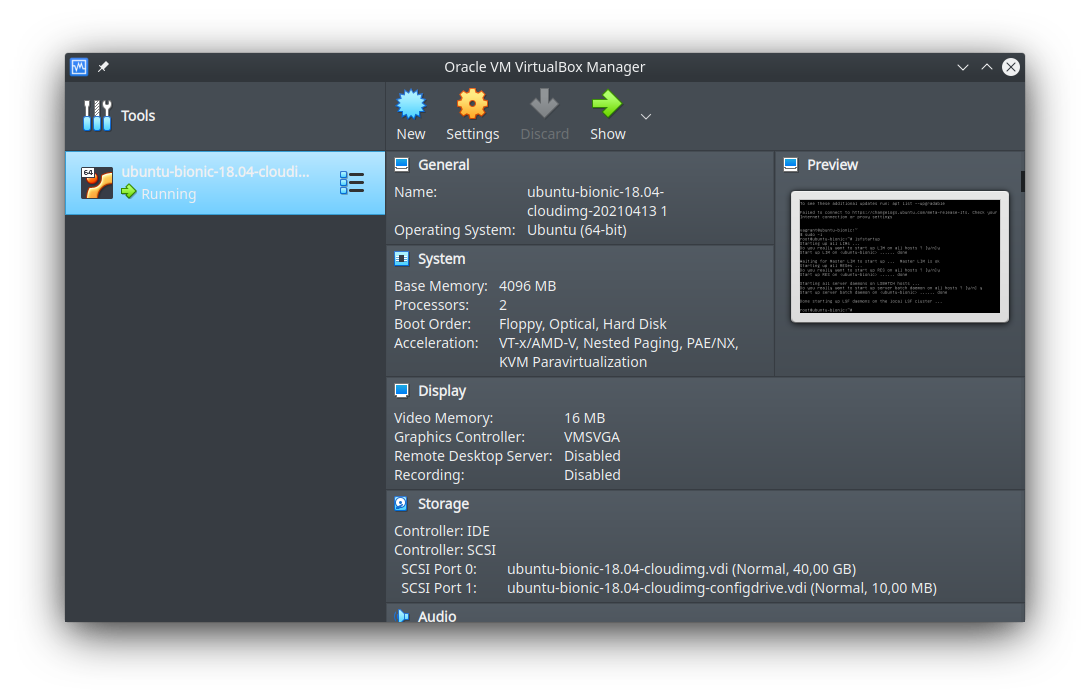
\includegraphics[width=\linewidth]{vbox.png}
    \caption{VirtualBox}
    % \label{fig:block-scheme}
\end{figure}

\begin{figure}[h]
    \centering
    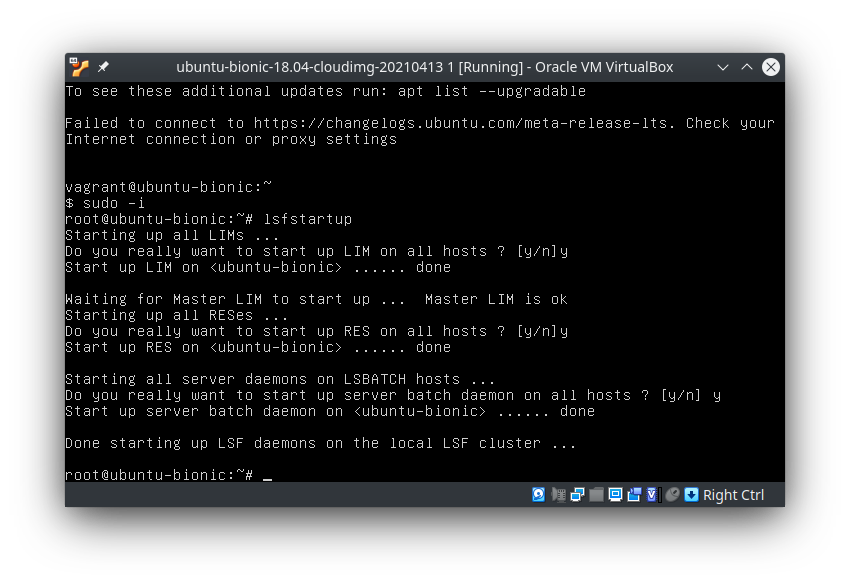
\includegraphics[width=\linewidth]{vm.png}
    \caption{Виртуальная машина. Изображен запуск LSF}
    % \label{fig:block-scheme}
\end{figure}

\begin{figure}[h]
    \centering
    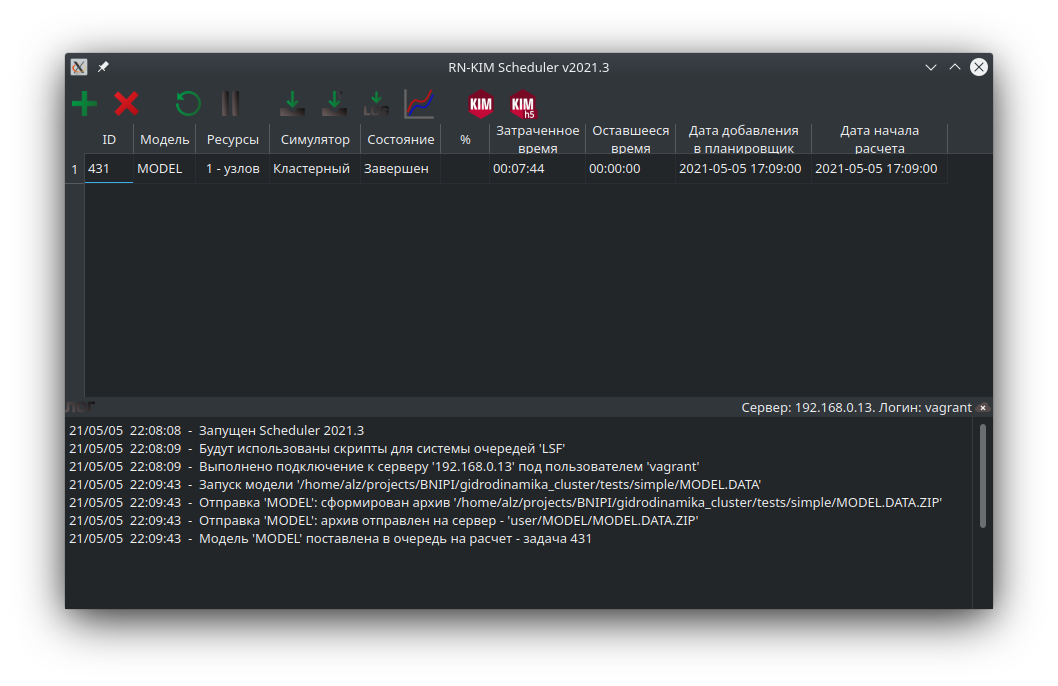
\includegraphics[width=\linewidth]{type_cluster.png}
    \caption{Скриншот Scheduler. Тип расчета модели: кластерный}
    % \label{fig:block-scheme}
\end{figure}

\begin{figure}[h]
    \centering
    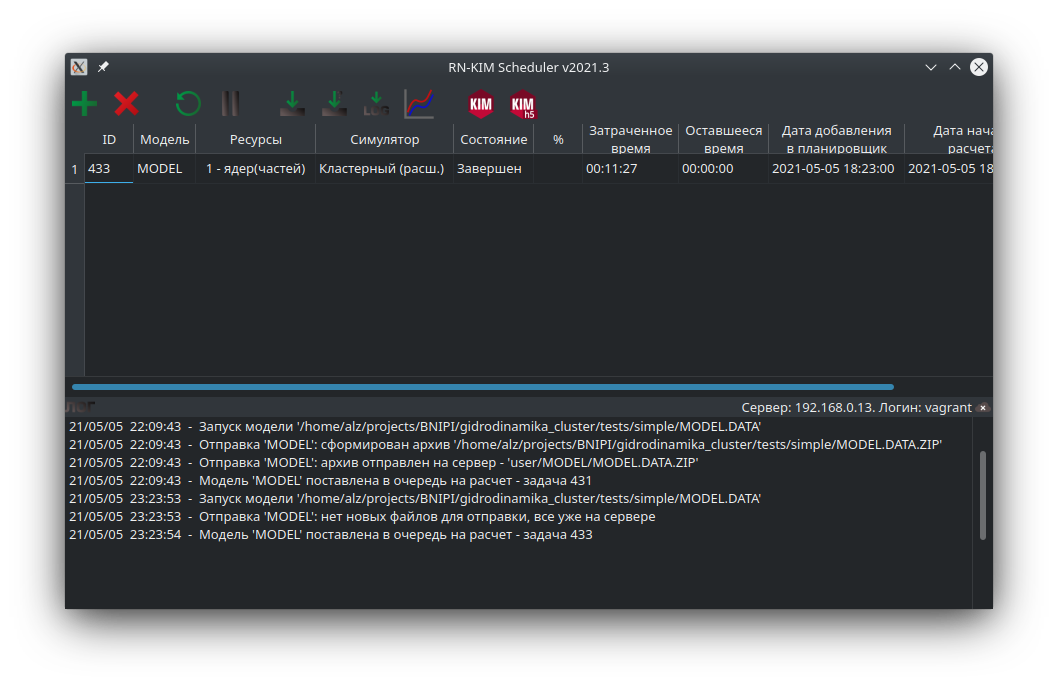
\includegraphics[width=\linewidth]{type_cluster_expanded.png}
    \caption{Скриншот Scheduler. Тип расчета модели: кластерный (расш.)}
    % \label{fig:block-scheme}
\end{figure}

\begin{figure}[h]
    \centering
    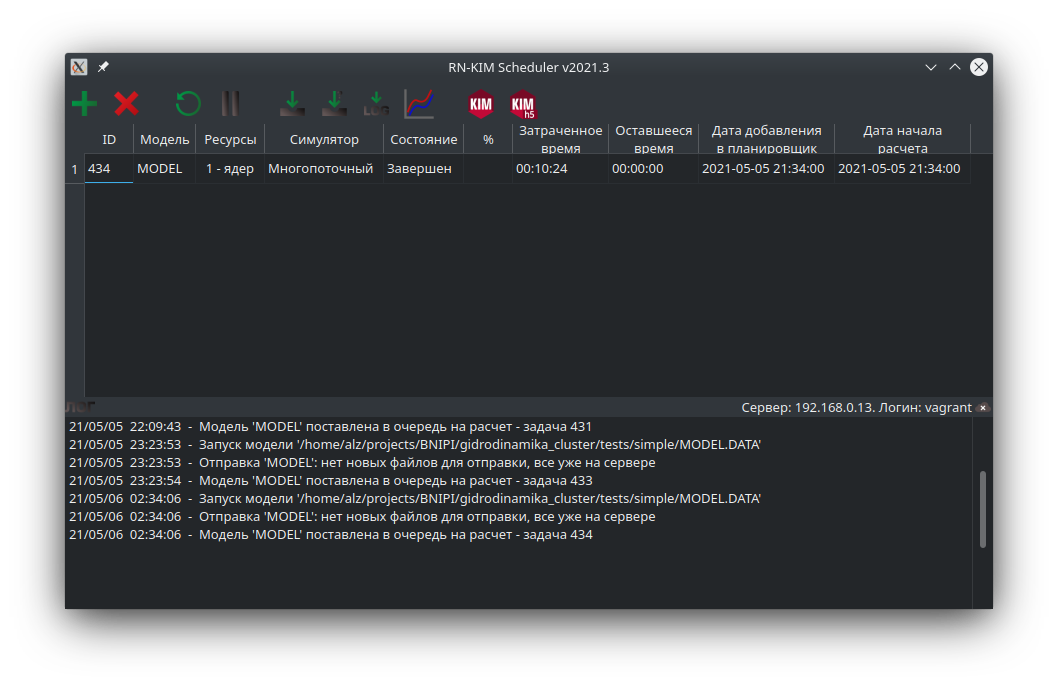
\includegraphics[width=\linewidth]{type_multithread.png}
    \caption{Скриншот Scheduler. Тип расчета модели: многопоточный}
    % \label{fig:block-scheme}
\end{figure}

\begin{figure}[h]
    \centering
    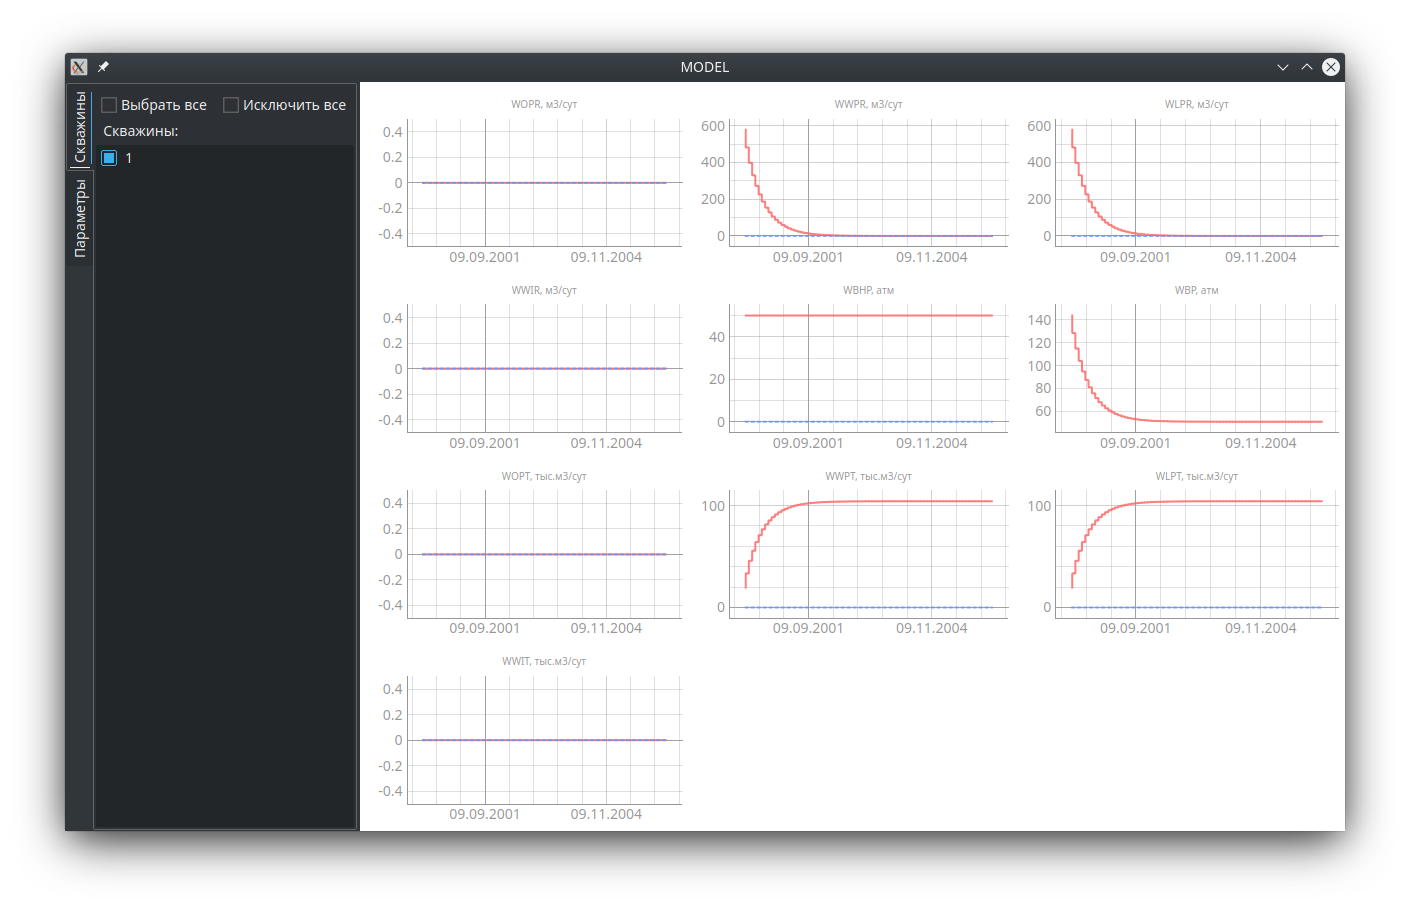
\includegraphics[width=\linewidth]{curves.png}
    \caption{Скриншот Scheduler. Рассчитанные кривые модели}
    % \label{fig:block-scheme}
\end{figure}

\clearpage